\section{Sisteme de recomandare}

\subsection{Noțiuni generale}

Sistemele de recomandare au scopul de oferi sugestii de articole utilizatorilor unei platforme pe baza unor strategii. Un sistem de recomandare poate folosi una sau mai multe strategii de recomandare. 

În cazul în care se folosesc cel puțin două strategii, sistemul de recomandare devine un sistem de recomandare hibrid. Prin folosirea mai multor strategii se urmărește ca fiecare strategie să vină în completarea celorlalte cu avantajele sale.

De cele mai multe ori, în implementarea unui sistem de recomandare, se folosește tehnica de filtrare coloborativă împreună cu o altă strategie de recomandare \hyperlink{ErionCanoMaurizioMorisio}{[4]}.

\subsection{Strategii de recomandare}

\subsubsection*{Filtrarea coloborativă}

Filtrarea coloborativă se bazează pe faptul că utilizatorii care au în prezent preferințe similare vor avea și în viitor preferințe destul de similare. Această abordare folosește ratingurile pe care le dau utilizatorii sau oricare altă formă de a da un feedback, îmi place/nu îmi place, pentru a identifica preferințele comune dintre grupurile de utilizatori. Odată identificate preferințele se generează recomandări pe baza similarităților dintre utilizatori. 

Dezavantajul acestei strategii apare în momentul în care în sistem intră un nou utilizator. Datorită faptului că utilizatorul este nou, sistemul nu are un istoric al preferințelor lui, iar în consecință nu îl poate asigna unui grup de utilizatori pe baza preferințelor \hyperlink{ErionCanoMaurizioMorisio}{[4]}.

\begin{figure}[!h]
	\centering
	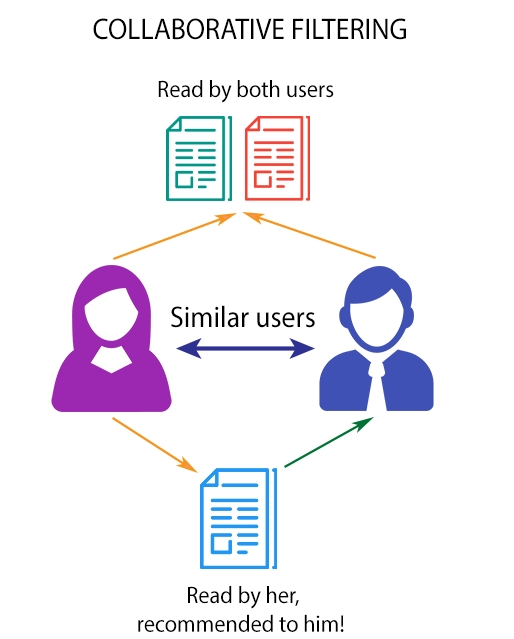
\includegraphics[max width=10cm,max height=10cm,keepaspectratio]{img_2_1}
	\caption[Filtrarea coloborativă]{Filtrarea coloborativă. Imagine preluată din \hyperlink{datameetsmedia}{[5]}.}
\end{figure} 

\subsubsection*{Filtrarea bazată pe conținut}

Filtrarea bazată pe conținut pleacă de la premisa că utiliztorii cărora le-au plăcut articole definite de anumite atribute în trecut, vor aprecia aceleași tip de articole și în viitor. Această abordare folosește atributele articolelor pentru a le compara cu profilul utilizatorilor și a oferi recomandări. Calitatea recomandărilor create folosind această strategie este influențată de setul de atribute ales pentru articole.

Similar cu filtrarea coloborativă și filtrarea bazată pe conținut prezintă dezavantaje în momentul în care în sistem intră un nou utilizator fără istoric \hyperlink{ErionCanoMaurizioMorisio}{[4]}.

\begin{figure}[!h]
	\centering
	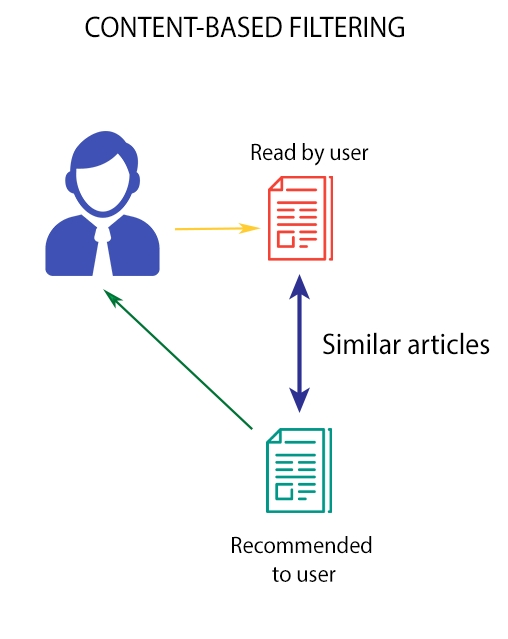
\includegraphics[max width=10cm,max height=10cm,keepaspectratio]{img_2_2}
	\caption[Filtrarea bazată pe conținut]{Filtrarea bazată pe conținut. Imagine preluată din \hyperlink{datameetsmedia}{[5]}.}
\end{figure} 

\subsubsection*{Filtrarea demografică}

Filtrarea demografică folosește atribute precum vârsta, genul, educația, etc. pentru a identifica categoriile de utilizatori. Nu prezintă dezavantaje atunci când apar noi utilizatori în sistem și nu se folosește de ratinguri, sau alt sistem de feedback, pentru a face recomandări.

Dezavantajul este reprezentat de faptul că procesul de colectare al datelor demografice poate fi îngreunat de legislație fapt ce reprezintă o limitare a acestei metode \hyperlink{ErionCanoMaurizioMorisio}{[4]}.

\subsubsection*{Filtrarea bazată pe cunoștințe}

Filtrarea bazată pe cunoștințe folosește cunoștințele despre utilizatori și articole pentru a spune ce articole îndeplinesc cerințele utilizatorilor și genereaza recomandări în consecință. Filtrare bazată pe cunoștințe are la bază constrângeri și este capabilă să recomande chiar și articole complexe care nu sunt cumpărate atât de des, precum mașini sau case \hyperlink{ErionCanoMaurizioMorisio}{[4]}.

\subsection{Funcții de loss}

\subsubsection*{BPR: Bayesian Personalised Ranking}

Maximizează diferența de predicției dintre un exemplu pozitiv și un exemplu negativ ales aleator. Este utilă atunci când sunt prezente doar interacțiuni pozitive și se dorește optimizarea acurateții \hyperlink{lighfm}{[6]}.

\subsubsection*{WARP: Weighted Approximate-Rank}

Maximizează rangul exemplelor positive prin eșantionarea repetată a exemplelor negative până când se constată o încălcare a rangului. Este utilă atunci când sunt prezente doar interacțiuni pozitive și se dorește optimizarea preciziei@k \hyperlink{lighfm}{[6]}.

\section{Rețele convoluționale}

\subsection{Noțiuni generale}

\subsection{VGG}

\subsection{InceptionV3}

\subsection{ResNet}

\subsection{NASNet}



\section{Clustere}

\subsection{Noțiuni generale}

\subsection{K-nearest neighbors}
